\documentclass[12pt,letterpaper]{article}
\usepackage[utf8]{inputenc}
\usepackage{amsmath}
\usepackage{amsfonts}
\usepackage{amssymb}
\usepackage{graphicx}
\usepackage{float}
\usepackage{vmargin}
\title{Aproximación Funcional e Interpolación}
\date{7 de Diciembre del 2018}

\setpapersize{A4}
\setmargins{2.5cm}       % margen izquierdo
{0cm}                        % margen superior
{16.5cm}                      % anchura del texto
{23.42cm}                    % altura del texto
{10pt}                           % altura de los encabezados
{1cm}                           % espacio entre el texto y los encabezados
{0pt}                             % altura del pie de página
{2cm}                           % espacio entre el texto y el pie de página

\begin{document}

\maketitle

\section{Introducción}
La enorme ventaja de aproximar información discreta o funciones “complejas” con funciones analíticas sencillas, radica en su mayor facilidad de evaluación y manipulación, situación necesaria en el campo de la ingeniería.
Las funciones de aproximación se obtienen por combinaciones lineales de elementos de familias de funciones denominadas elementales. 

Sea una función f(x), dada en forma tabular
\begin{figure}[hbtp]
\centering
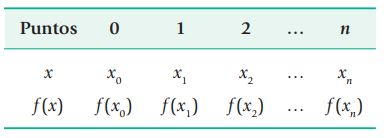
\includegraphics[scale=1]{imagenes/funcion.JPG}
\caption{Funcion tabulada}
\end{figure}

Para aproximar a la función modelo por medio de un polinomio se aplica el método de regresión y si quieres saber un punto en un rango y tienes muy pocos puedes hacer una interpolación en el parámetro que deseas encontrar tu valor en el gráfico.

\begin{figure}[hbtp]
\centering
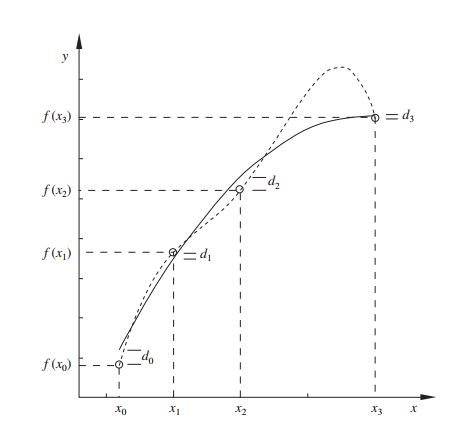
\includegraphics[scale=.4]{imagenes/ajuste.JPG}
\caption{Encuentras una función que se ajuste al modelo de regresión por mínimos cuadrados}
\end{figure}
\section{Objetivo}
Implementar los algoritmos para determinar los datos faltantes, analizar y comparar el desempeño de los diversos algoritmos y determinar cuando es mejor utilizar cada algoritmo en función de su desempeño y las características de los datos del problema
\section{Diseño Conceptual y resolución de puntos}
\subparagraph{Regresión por mínimos cuadrados}
La regresión por mínimos cuadrados es el método más común utilizado en la obtención de funciones de aproximación de un modelo con muchos puntos que indican un comportamiento ya sea lineal o no lineal, dependiendo del problema es el caso de mínimos cuadrados a utilizar.\\
Si el modelo representa un incremento o decremento lineal se usa la ecuación de la recta, a partir de ella buscaremos los coeficientes ideales para crear el modelo matemático que prediga puntos en el gráfico que no poseemos.

\begin{equation}
y=a_0+a_1x
\end{equation}
\begin{equation}
a_1=\frac{n \sum_{}^{} x_iy_ i -  \sum_{}^{} x_i \sum_{y_i}}{n\sum_{}^{} x_i^2- (\sum_{}^{} x_i)^2}
\end{equation}
\begin{equation}
a_0= \overline{y} - a_1  \overleftarrow{x}
\end{equation}

Si deseas hacer un modelo cuadrado o de n grado puedes usar el modelo generalizado de crear tu sistema de ecuaciones representado en una matriz para resolver las $a_i$ hasta $a_n$ por medio del método de Gauss Jordan.

\[ I^{n \times n} =
\left( \begin{array}{cccc}
 d & \sum_{}^{}1 x & \cdots & \sum_{}^{} x^n \\ 
 \sum_{}^{}x & \sum_{}^{} x^2 & \cdots & \sum_{}^{} x^{n+1} \\
 \vdots & \vdots & \ddots & \vdots \\
 \sum_{}^{} x^n & \sum_{}^{} x^{n+1} & \cdots & ...
\end{array} \right) \]
 \subsubsection{Punto 2}
 \begin{figure}[hbtp]
 \centering
 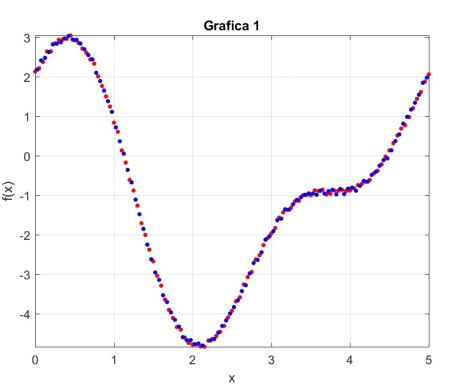
\includegraphics[scale=.7]{imagenes/modelo2.JPG}
 \caption{Modelo}
 \end{figure}
 
Suponga que la funcion f(x) mostrada por la figura 2 es la respuesta de un
sensor a la entrada x, los puntos en rojos que estan guardados en el archivo Datos 1 1.txt pueden ser utilizados para obtener un modelo y los datos en azul que
estan guardados en el archivo Datos 1 2.txt puede ser utilizados para comprobar
el modelo. Se desea obtener un modelo suponiendo los siguientes casos:\\
a. Realice una regresion por minimos cuadrados en todo el rango de los datos
suponiendo un modelo lineal.\\
b. Realice una regresion por mınimos cuadrados en n segmentos en el rango
de los datos suponiendo un modelo lineal. Considere que el valor de n debe
ser el optimo para mınimizar el error cuadratico medio.\\
c. Realice un regresion por mınimos cuadrados en todo el rango de los datos
suponinendo un modelo cuadratico.\\
d. Realice una regresion por mınimos cuadrados en n segmentos en el rango
de los datos suponiendo un modelo cuadratico. Considere que el valor de
n debe ser el optimo para mınimizar el error cuadratico medio.\\
e. Realice un regresion por mınimos cuadrados en todo el rango de los datos
suponinendo un modelo cubico.\\

f. Realice una regresion por mınimos cuadrados en n segmentos en el rango
de los datos suponiendo un modelo cubico. Considere que el valor de n
debe ser el optimo para mınimizar el error cuadratico medio.\\
g. Realice un analisis comparativo entre los modelos lineal, cuadratico y cubico para todo el rango de los datos y explique sus resultados.\\
h. Realice un analisis comparativo entre los modelos lineal, cuadratico y cubico para el comportamiento de los n segmentos y explique sus resultados.\\
i. Realice un analisis comprativo entre todos los modelos obtenidos y explique sus resultados.\\

Resolución:
-Se implemento el manejo de $Datos-1-1. txt$ en matlab a modo de matriz de 2 renglones por 101 columnas.\\
-Para visualizar el modelo se llevo a cabo un "plot" de los datos tomando como $x$ la fila 1 y como $y$ la fila 2.\\
-Se visualizó el modelo\\
-Se llevan a cabo la resolución de las ecuaciones antes mencionadas \\
. \quad -Para ello se separan en dos vectores fila la matriz con las coordenadas dentro de un for\\
. \quad -Se hace una evaluación de las sumatorias diversas\\
. \quad -Se hacen las ecuaciones pertinentes en la regresión lineal y la resolución de ecuaciones en la regresión cuadrada y cúbica por medio de Gauss Jordan.\\
-Una vez obtenidas las $a_o,a_1,....,a_n$ se procede a sustituirlas en la ecuación del modelo calculado.\\
-Se hace le "plot()" de las ecuaciones y se hacen las comparaciones con el modelo original.\\

\subparagraph{Interpolación en una dimensión}
.\\
La interpolación es de gran importancia en el campo de la ingeniería, ya que al consultar fuentes de
información presentadas en forma tabular, con frecuencia no se encuentra el valor buscado como un
punto en la tabla. Por ejemplo, la temperatura de ebullición de la acetona $(C3H6O)$ a diferentes presiones.
\begin{figure}[hbtp]
\centering
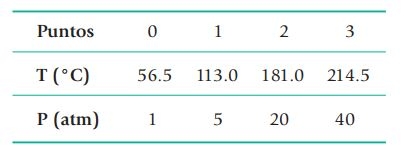
\includegraphics[scale=1]{imagenes/presiones.JPG}
\caption{Presiones de la acetona a diferentes presiones}
\end{figure}
Una forma muy común de resolver este problema es sustituir los puntos (0) y (1) en la ecuación
de la línea recta: p (x) = a0 + a1x, de tal modo que resultan dos ecuaciones con dos incógnitas que son
a0 y a1. \\

\begin{equation}
56.5+a_0+a_1
\end{equation}
Y sustituimos el punto 1
\begin{equation}
113=a_0+5a_1
\end{equation}
y si resolvemos el sistema da a0 = 42.375 y a1 = 14.125\\
Con la solución del sistema se consigue una aproximación polinomial de primer grado, lo que
permite efectuar interpolaciones lineales; es decir, se sustituye el punto (0) en la ecuación de la línea
recta y se obtiene:
\begin{equation}
p(x)=42.375+14.125x
\end{equation}
La ecuación resultante puede emplearse para aproximar la temperatura cuando la presión es conocida.
Al sustituir la presión x = 2 atm, se obtiene una temperatura de 70.6 C. A este proceso se le conoce como interpolación.
\begin{figure}[hbtp]
\centering
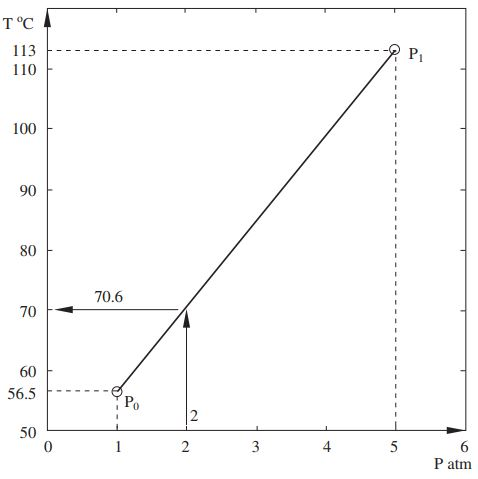
\includegraphics[scale=.5]{imagenes/interpolacion.JPG}
\caption{Resultado de la interpolación de los puntos de ebullición, se obtiene una ecuación que puede describir algunos puntos no conocidos.}
\end{figure}

\subparagraph{Interpolación en dos dimensiones}

\section{Resultados y Conclusiones}

\subsection{Punto2}
\begin{figure}[hbtp]
\centering
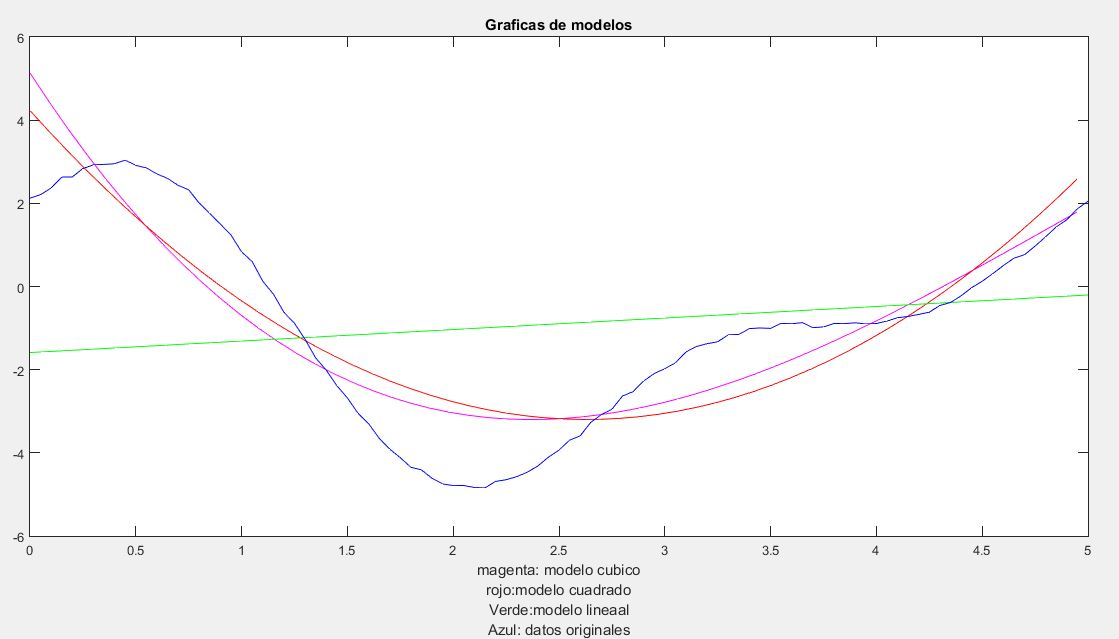
\includegraphics[scale=.5]{imagenes/resolucion2.JPG}
\caption{Comparando cada uno de los modelos con los daros originales}
\end{figure}
La utilización de cada uno des los métodos de regresión lineal por mínimos cuadrados fue satisfactoria de acuerdo a cada modelo, se puede observar una notable mejora del modelo lineal al saltar al modelo cuadrado (como era de esperarse debido que el los datos no se comportan de manera lineal), sin embargo, del salto del modelo cuadrado al modelo cúbico solo se da un pequeño ajuste de curva muy mínimo, lo que se sospecha que se necesita un polinomio de grado muy alto para que tienda a un error cuadrático medio muy bajo.


a\\ \\
Referencias:
Métodos Numéricos para Ingenieros. Quinta Edición, Steven C. Chapra  \\
http://www-history.mcs.st-andrews.ac.uk/Biographies/Raphson.html

\end{document}